\chapter{Нейросетевые модели управления технологическими процессами}

В данной главе рассматриваются практические примеры применения в задачах АСУТП.

\section{Процесс пастеризации молока}

\subsection{Общие сведения}

К концу XIX века тепловая обработка молока получила столь широкое применение, что стала использоваться для разнообразных целей на большинстве молокозаводов – например, для обработки молока при изготовлении сыра и масла. До внедрения тепловой обработки молоко представляло собой постоянный источник инфекций, так как оно является идеальной средой для развития микроорганизмов. Через молоко зачастую распространялись такие болезни, как туберкулез и брюшной тиф.

В термине “пастеризация” запечатлено имя Луи Пастера, который в середине XIX века провел фундаментальные исследования воздействия тепла на микроорганизмы, приводящего к их гибели, и возможности применения температурной обработки для консервирования пищевых продуктов.

Пастеризация молока – это особый вид тепловой обработки, который можно определить как “любую тепловую обработку молока, обеспечивающую безусловное уничтожение микроорганизмов – возбудителей туберкулеза, не вызывая при этом значительных изменений физических и химических качеств молока” \cite{TetraPak1995}.

Пластинчатая пастеризационно-охладительная установка (ПОУ) предназначена для тепловой обработки и охлаждения молочных продуктов в непрерывном тонкослойном закрытом потоке. Схема типовой пастеризационной установки приведена ниже (рис. \ref{fig:POU_Tetra_Pak}). Нагрев осуществляется за счет подачи пара через управляемый клапан \textbf{VC1}. Диапазон работы управляемых паровых клапанов от $\text{0\%}$ – полностью закрыт, до $\text{100\%}$ – полностью открыт. Температура \textbf{TE1} поддерживаться в пределах $92 \pm 2 \SI{}{\celsius}$.

Современная ПОУ, включающая оборудование для эксплуатации, надзора и управления процессом, собирается из согласованных компонентов, образуя сложный технологический агрегат. Для автоматизации регулирования температурного режима в состав ПОУ входит система управления на базе промышленного контроллера. От применяемых алгоритмов управления напрямую зависит качество получаемой продукции.

\begin{figure}[H]
    \centering
    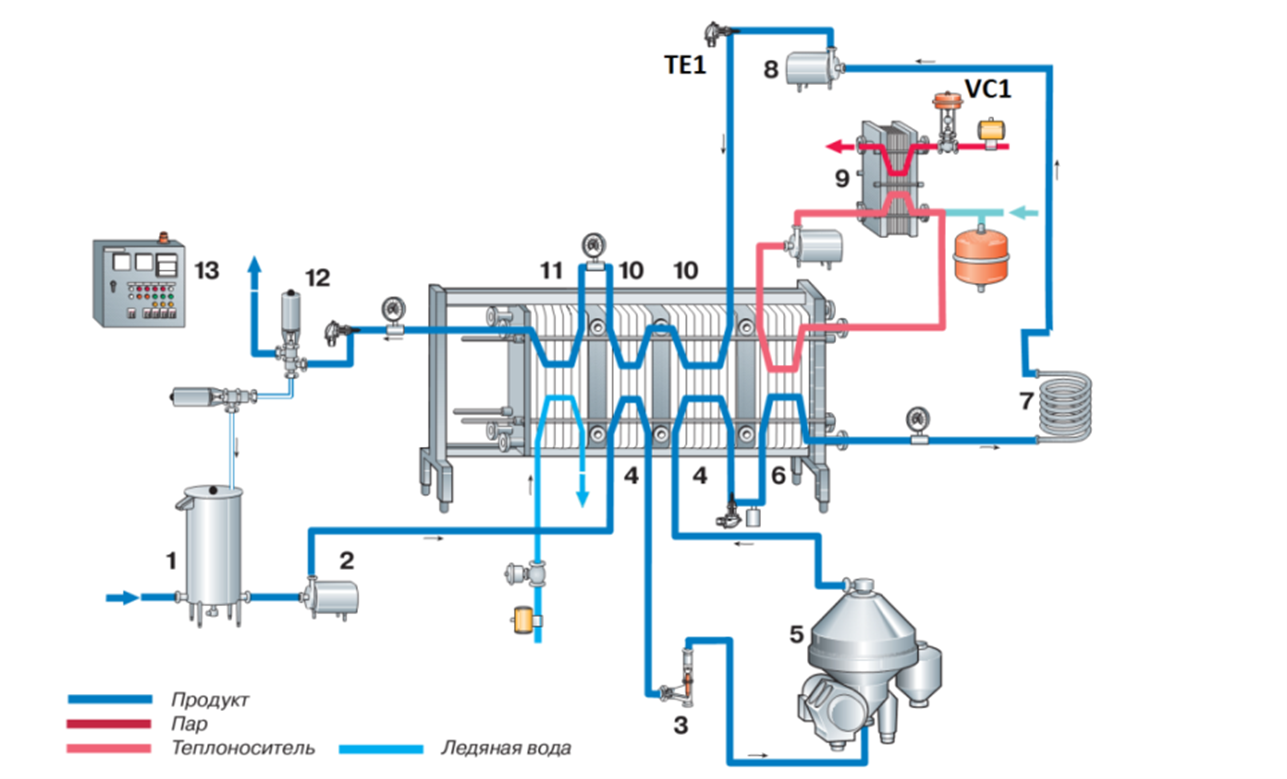
\includegraphics[width=\textwidth]{images/chapter_2/ПОУ Tetra Pak.png}
    \caption{Схема и общий вид пастеризационной установки, где: 1 - балансный танк, 2 - подающий насос, 3 - регулятор потока, 4 - секции регенеративного предварительного подогрева, 5 - центробежный очиститель, 6 - секция нагрева, 7 - труба выдержки, 8 - вспомогательный насос, 9 - система нагрева горячей воды, 10 - секции регенеративного охлаждения, 11 - секции охлаждения, 12 - клапан возвратный, 13 - панель управления}
    \label{fig:POU_Tetra_Pak}
\end{figure}

\subsection{Пастеризационные установки как объект автоматизации}

Рассмотрим подробно секцию нагрева ПОУ. Входные и выходные параметры и возмущающие воздействия для нее представлены на рис. \ref{fig:Pasterizer_heat_section}.

\begin{figure}[H]
    \centering
    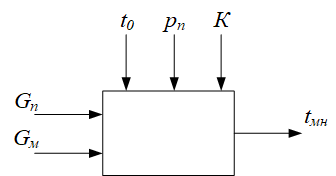
\includegraphics{images/chapter_2/Pasterizer_heat_section.png}
    \caption{Структурная схема секции нагрева ПОУ как объекта автоматизации}
    \label{fig:Pasterizer_heat_section}
\end{figure}

Основными причинами, вызывающими колебания температуры $t_\text{мн}$ нагревания молока являются непостоянство расхода $G_\text{м}$ продукта, непостоянство температуры $t_0$ исходного молока, изменение расхода $G_\text{п}$ пара, обусловленное колебания его давления $p_\text{п}$, изменение коэффициента теплопередачи $K$ вследствие отложения белка молока на теплопередающих поверхностях \cite{Вайнберг1978}.

Для стабилизации температуры $t_\text{мн}$ нагревания молока в качестве управляющего воздействия в основном применяют расход пара $G_\text{п}$. Его регулируют посредством управляемого клапана (\textbf{VC1} на рис. \ref{fig:Pasterizer_heat_section}).

Статические и динамические характеристики большинства ПОУ в настоящее время экспериментально и аналитически выявлены. Для нагревательной части по каналу $G_\text{п} \rightarrow t_\text{мн}$, т. е. зависимость $t_\text{мн}=F(G_\text{п})$ определяется из уравнения теплового баланса секции пастеризации и систем обогрева горячей воды. Если пренебречь потерями тепла в окружающую среду, то уравнение теплового баланса в установившемся режиме имеет вид:

\begin{equation}
    G_\text{м} c_\text{м}(1 - \varepsilon)(t_\text{мн} - t_0) = G_\text{п}(i - c_\text{к} t_\text{к}),
\end{equation}

где $c_\text{к}$ – температура конденсата \SI{}{\celsius}; $c_\text{м}$, $c_\text{к}$ – теплоемкость соответственно молока и конденсата, Дж/(кг·\SI{}{\celsius}); $\varepsilon$ – коэффициент регенерации тепла установки; $i$ – энтальпия пара, Дж/кг. После преобразования данного уравнения получаем статическую характеристику нагревательной части установки:

\begin{equation}
    t_\text{мн} = t_0 + \frac{i - c_\text{к} t_\text{к}}{G_\text{м} c_\text{м}(1 - \varepsilon)} G_\text{п}.
\end{equation}

Результаты экспериментальных и теоретических исследований показали, что динамическая характеристика нагревательной части установки по каналу «расход пара – температура нагрева молока» может быть выражена передаточной функцией:

\begin{equation}\label{steam_temp_relation}
    W(p) = \frac{K_\text{п} e^{-p \tau_\text{з}}} {Tp + 1},
\end{equation}

где $K_\text{п}$ – коэффициент передачи объекта, \SI{}{\celsius}/(кг/с),

\begin{equation}
    K_\text{п} = \frac{i - c_\text{к} t_\text{к}}{G_\text{м} c_\text{м}(1 - \varepsilon)},
\end{equation}

где $T$ – постоянная времени объекта, с; $\tau_\text{з}$ – время запаздывания, с; $p$ – комплексная переменная (оператор Лапласа).

Таким образом, передаточная функция нагревательной части установки характеризуется последовательно соединенными апериодическим звеном первого порядка и звеном транспортного запаздывания. В таблице \ref{table:pasterizer_params} приведены средние значения параметров некоторых ПОУ.

\begin{table} [!h]
    \small
    \caption{Параметры ПОУ}\label{table:pasterizer_params}
    \centering
    \begin{tabular}{ | c | c | c | c | }
        \hline
        \textbf{Установка} & $K_\text{п}$, \SI{}{\celsius}/(кг/с) & $T$, c & $\tau_\text{з}$, c \\
        \hline
        ОПУ-5М             & 2300                                 & 369    & 12                 \\
        \hline
        ОПУ-10             & 1150                                 & 190    & 7                  \\
        \hline
        ОПУ-25             & 525                                  & 450    & 4                  \\
        \hline
    \end{tabular}
\end{table}

При накоплении белковых веществ на теплопередающих поверхностях значения $T$ в среднем возрастают на 50 - 60\%.

\subsection{Компьютерное моделирование процесса пастеризации}

Для компьютерного моделирования получим дискретную модель процесса пастеризации на основе формулы (\ref{steam_temp_relation}).

Рассмотрим процесс без участия звена запаздывания $e^{-p \tau_\text{з}}$, положим $k = K_\text{п}$. Выберем достаточно малый шаг времени $h$ и будем вычислять значения сигналов на выходе в дискретные равноотстоящие моменты времени $t = hl$ $(l = 0, 1, 2, \ldots)$. Выходную величину определим по рекуррентным формулам квадратичной интерполяции на основе значений сигнала, полученных в предыдущие моменты времени. Дифференциальное уравнение процесса в интервале $(l - 1)h < t \le hl$ имеет вид:

\begin{equation}
    Tdy(\tau)/d\tau + y(\tau) = kx(\tau),
\end{equation}

где $\tau = t - (l - 1)h$.

При $\tau = 0$ значения $x[(l - 1)h] = x_{l - 1}, y[(l - 1)h] = y_{l - 1}$.

Переходя к изображениям по Лапласу и решая уравнение относительно $Y(p)$, получим:

\begin{equation}
    Y(p) = \frac{1}{1 + pT}y_{l - 1}+\frac{k}{1 + pT}[X(p) - x_{l - 1}].
\end{equation}

При использовании квадратичной интерполяции сигнал $x(t)$ в интервале $[(l - 1)h, lh]$ определяется значениями $x$ для трех моментов времени $x_l = x(lh), x_{l - 1} = x[(l - 1)h)]$ и $x_{l - 2} = x[(l - 2)h)]$, т.е.:

\begin{equation}
    x(t) = x_{l - 1} + \frac{x_l - x_{l - 2}}{2h} + \frac{x_l - 2x_{l - 1}+ x_{l - 2}}{h^2},
\end{equation}

или в изображениях:

\begin{equation}
    x(p) = \frac{x_{l - 1}}{p} + \frac{x_l - x_{l - 2}}{2h}\cdot\frac{1}{p^2} + \frac{x_l - 2x_{l - 1} + x_{l - 2}}{h^2}\cdot\frac{1}{p^3}.
\end{equation}

Выполняя подстановку и обратное преобразование Лапласа, при $\tau = h$, т.е. в конце интервала $(t = lh)$, имеем:

\begin{equation}
    y_l = \gamma y_{l - 1} + Ax_l + Bx_{l - 1} + Cx_{l - 2},
\end{equation}

где:

\begin{equation}
    \begin{rcases}
        \gamma = e^{-h/T};\\
        A = \frac{k}{2h^2}[(1 - \gamma)(2T^2 - Th) + 2h^2 - 2Th];\\
        B = -\frac{k}{h^2}[(1 - \gamma)(2T^2 - h^2) + h^2 - 2Th];\\
        C = \frac{k}{2h^2}[(1 - \gamma)(2T^2 + Th) - 2Th].
    \end{rcases}
\end{equation}

С учетом запаздывания $\tau_\text{з}$ получим \cite{Нетушил1978}:

\begin{equation}
    y_l = \gamma y_{l - 1} + Ax_{l - \tau_\text{з}} + Bx_{l - \tau_\text{з} - 1} + Cx_{l - \tau_\text{з} - 2}.
\end{equation}.

\subsection{Разработанный нейро-ПИД регулятор ПОУ}

Общая структура самонастраивающегося нейро-ПИД регулятора показана на рисунке \ref{fig:neuro_PID_controller}, где выходы нейронной сети – пропорциональный ($K_P$), интегральный ($K_I$) и дифференциальный ($K_D$) коэффициенты.

\begin{figure}[H]
    \centering
    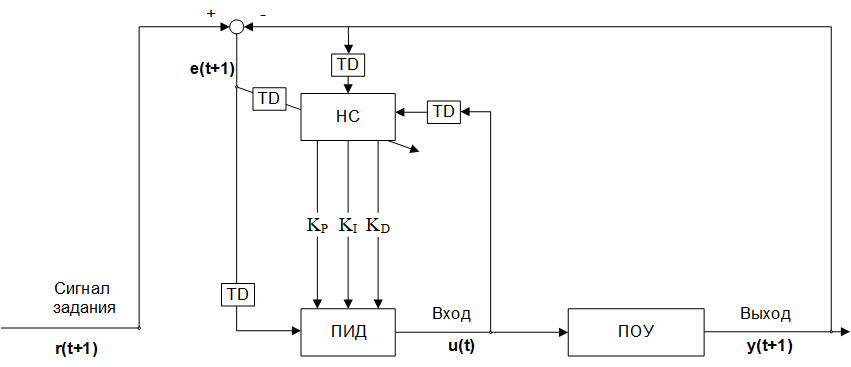
\includegraphics[width=\textwidth]{images/chapter_2/Разработанный нейро-контроллер.png}
    \caption{Разработанный нейро-ПИД-регулятор, TD означает оператор задержки}
    \label{fig:neuro_PID_controller}
\end{figure}

В качестве настройщика ПИД использовался многослойный персептрон (MLP) со следующей структурой: 20 входных, 10 скрытых и 3 выходных нейронных элемента; функция активации скрытого и выходного слоев – сигмоидная (рис. \ref{fig:PID_neuro_tuner}).

\begin{figure}[H]
    \centering
    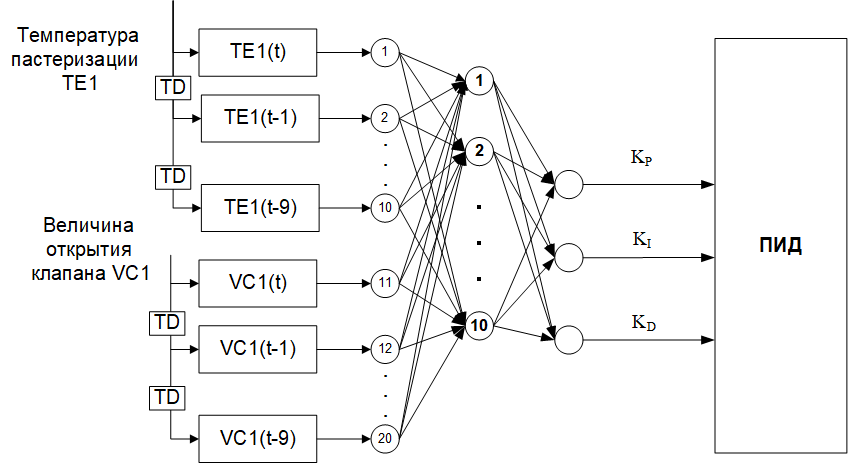
\includegraphics[width=\textwidth]{images/chapter_2/Нейро-настройщик ПИД.png}
    \caption{Нейро-настройщик ПИД}
    \label{fig:PID_neuro_tuner}
\end{figure}